\documentclass{standalone}
\usepackage{tikz}
\usetikzlibrary{patterns, positioning}
\usepackage[sfdefault]{ClearSans} %% option 'sfdefault' activates Clear Sans as the default text font
\usepackage[T1]{fontenc}

\begin{document}
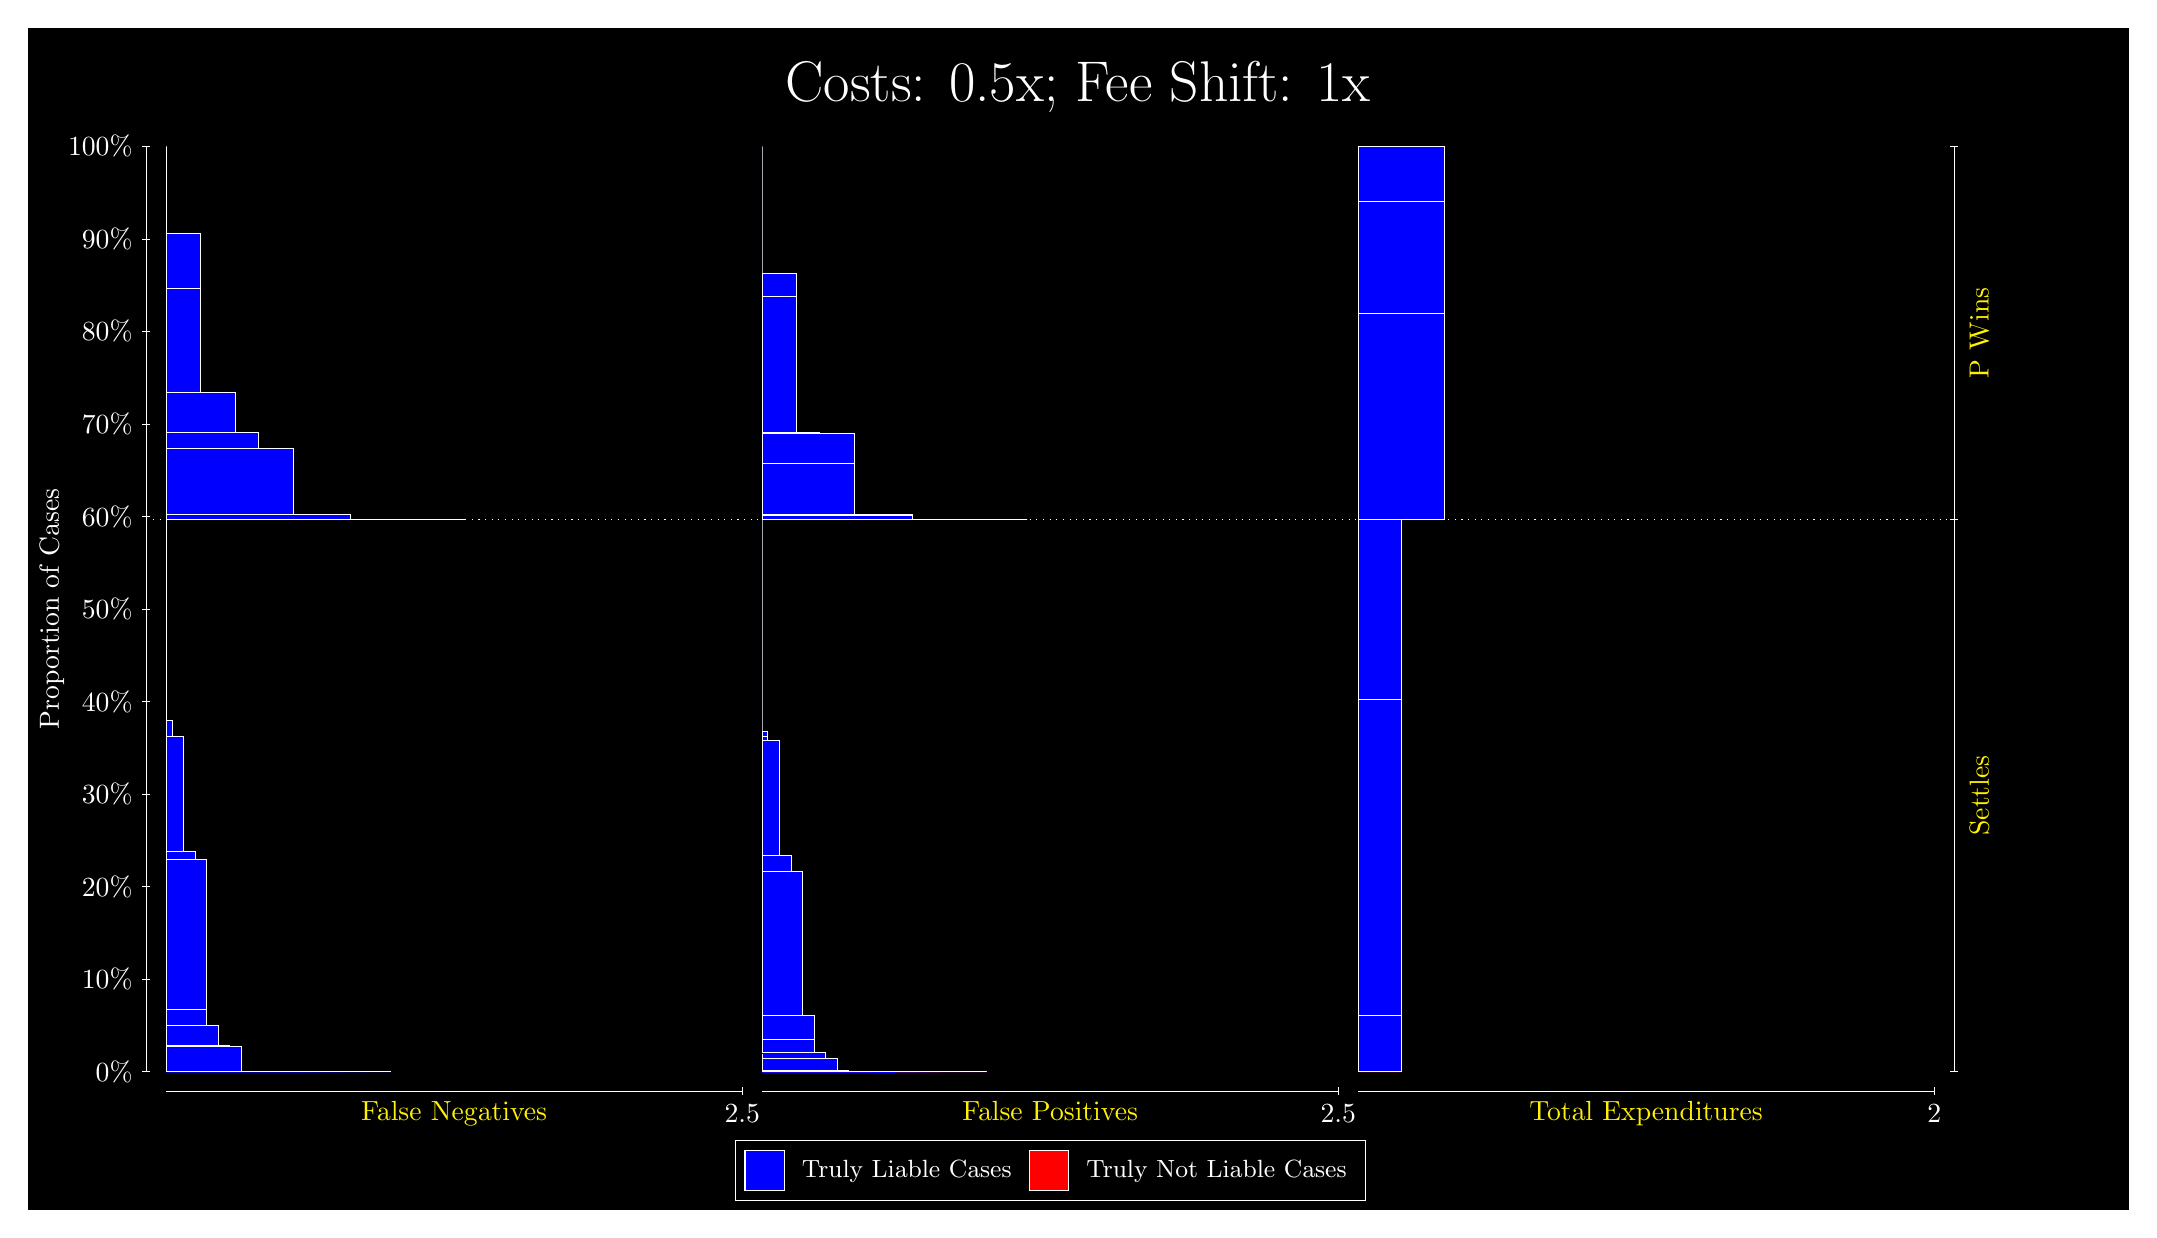
\begin{tikzpicture}
\draw[fill=black] (0,0) rectangle (26.667,15);
\draw[text=white] (0,13.5) rectangle (26.667,15) node[midway] {\huge Costs: 0.5x; Fee Shift: 1x};
\draw[white, very thin] (1.5,1.75) -- (1.5,13.5);
\node[rotate=90, text=white, anchor=center] at (0.3, 7.625) {Proportion of Cases};
\draw[white, very thin] (1.45,1.75) -- (1.55,1.75);
\node[text=white, anchor=east] at (1.45, 1.75) {0\%};
\draw[white, very thin] (1.45,2.925) -- (1.55,2.925);
\node[text=white, anchor=east] at (1.45, 2.925) {10\%};
\draw[white, very thin] (1.45,4.1) -- (1.55,4.1);
\node[text=white, anchor=east] at (1.45, 4.1) {20\%};
\draw[white, very thin] (1.45,5.275) -- (1.55,5.275);
\node[text=white, anchor=east] at (1.45, 5.275) {30\%};
\draw[white, very thin] (1.45,6.45) -- (1.55,6.45);
\node[text=white, anchor=east] at (1.45, 6.45) {40\%};
\draw[white, very thin] (1.45,7.625) -- (1.55,7.625);
\node[text=white, anchor=east] at (1.45, 7.625) {50\%};
\draw[white, very thin] (1.45,8.8) -- (1.55,8.8);
\node[text=white, anchor=east] at (1.45, 8.8) {60\%};
\draw[white, very thin] (1.45,9.975) -- (1.55,9.975);
\node[text=white, anchor=east] at (1.45, 9.975) {70\%};
\draw[white, very thin] (1.45,11.15) -- (1.55,11.15);
\node[text=white, anchor=east] at (1.45, 11.15) {80\%};
\draw[white, very thin] (1.45,12.325) -- (1.55,12.325);
\node[text=white, anchor=east] at (1.45, 12.325) {90\%};
\draw[white, very thin] (1.45,13.5) -- (1.55,13.5);
\node[text=white, anchor=east] at (1.45, 13.5) {100\%};

\draw[white, very thin] (24.457,1.75) -- (24.457,13.5);
\draw[white, very thin] (24.407,1.75) -- (24.507,1.75);
\node[anchor=west] at (24.407, 1.75) {};
\draw[white, very thin] (24.407,8.762) -- (24.507,8.762);
\node[anchor=west] at (24.407, 8.762) {};
\draw[white, very thin] (24.407,13.5) -- (24.507,13.5);
\node[anchor=west] at (24.407, 13.5) {};

\draw[white, very thin, fill=blue] (1.75,1.75) rectangle (4.6044,1.75);
\draw[white, very thin, fill=blue] (1.75,1.75) rectangle (4.3116,1.75);
\draw[white, very thin, fill=blue] (1.75,1.75) rectangle (4.0188,1.75);
\draw[white, very thin, fill=blue] (1.75,1.75) rectangle (3.8725,1.75);
\draw[white, very thin, fill=blue] (1.75,1.75) rectangle (3.7261,1.75);
\draw[white, very thin, fill=blue] (1.75,1.75) rectangle (3.5797,1.75);
\draw[white, very thin, fill=blue] (1.75,1.75) rectangle (3.4333,1.7507);
\draw[white, very thin, fill=blue] (1.75,1.7507) rectangle (3.287,1.7507);
\draw[white, very thin, fill=blue] (1.75,1.7507) rectangle (3.1406,1.7511);
\draw[white, very thin, fill=blue] (1.75,1.7511) rectangle (2.9942,1.7528);
\draw[white, very thin, fill=blue] (1.75,1.7528) rectangle (2.8478,1.756);
\draw[white, very thin, fill=blue] (1.75,1.756) rectangle (2.7015,2.0683);
\draw[white, very thin, fill=blue] (1.75,2.0683) rectangle (2.5551,2.0787);
\draw[white, very thin, fill=blue] (1.75,2.0787) rectangle (2.4087,2.3382);
\draw[white, very thin, fill=blue] (1.75,2.3382) rectangle (2.2623,2.5378);
\draw[white, very thin, fill=blue] (1.75,2.5378) rectangle (2.2623,4.4415);
\draw[white, very thin, fill=blue] (1.75,4.4415) rectangle (2.1159,4.5522);
\draw[white, very thin, fill=blue] (1.75,4.5522) rectangle (1.9696,6.0108);
\draw[white, very thin, fill=blue] (1.75,6.0108) rectangle (1.8232,6.215);
\draw[white, very thin, fill=red] (1.75,6.215) rectangle (1.75,6.215);
\draw[white, very thin, fill=blue] (1.75,6.215) rectangle (1.75,8.762);
\draw[white, very thin, fill=blue] (1.75,8.762) rectangle (5.5558,8.762);
\draw[white, very thin, fill=blue] (1.75,8.762) rectangle (4.8239,8.763);
\draw[white, very thin, fill=blue] (1.75,8.763) rectangle (4.3848,8.763);
\draw[white, very thin, fill=blue] (1.75,8.763) rectangle (4.092,8.8293);
\draw[white, very thin, fill=blue] (1.75,8.8293) rectangle (3.6529,8.8294);
\draw[white, very thin, fill=blue] (1.75,8.8294) rectangle (3.3602,9.6654);
\draw[white, very thin, fill=blue] (1.75,9.6654) rectangle (2.921,9.8703);
\draw[white, very thin, fill=blue] (1.75,9.8703) rectangle (2.6283,10.379);
\draw[white, very thin, fill=blue] (1.75,10.379) rectangle (2.1891,11.697);
\draw[white, very thin, fill=blue] (1.75,11.697) rectangle (2.1891,12.399);
\draw[white, very thin, fill=blue] (1.75,12.399) rectangle (1.8964,12.401);
\draw[white, very thin, fill=red] (1.75,12.401) rectangle (1.75,12.401);
\draw[white, very thin, fill=blue] (1.75,12.401) rectangle (1.75,13.5);
\draw[white, very thin, fill=red] (9.3189,1.75) rectangle (12.173,1.75);
\draw[white, very thin, fill=blue] (9.3189,1.75) rectangle (12.173,1.75);
\draw[white, very thin, fill=red] (9.3189,1.75) rectangle (11.588,1.75);
\draw[white, very thin, fill=blue] (9.3189,1.75) rectangle (11.588,1.75);
\draw[white, very thin, fill=blue] (9.3189,1.75) rectangle (11.441,1.75);
\draw[white, very thin, fill=red] (9.3189,1.75) rectangle (11.295,1.75);
\draw[white, very thin, fill=blue] (9.3189,1.75) rectangle (11.295,1.75);
\draw[white, very thin, fill=red] (9.3189,1.75) rectangle (11.002,1.75);
\draw[white, very thin, fill=blue] (9.3189,1.75) rectangle (11.002,1.7503);
\draw[white, very thin, fill=blue] (9.3189,1.7503) rectangle (10.856,1.7503);
\draw[white, very thin, fill=red] (9.3189,1.7503) rectangle (10.709,1.7503);
\draw[white, very thin, fill=blue] (9.3189,1.7503) rectangle (10.709,1.7507);
\draw[white, very thin, fill=blue] (9.3189,1.7507) rectangle (10.709,1.7512);
\draw[white, very thin, fill=blue] (9.3189,1.7512) rectangle (10.563,1.7512);
\draw[white, very thin, fill=red] (9.3189,1.7512) rectangle (10.417,1.7512);
\draw[white, very thin, fill=blue] (9.3189,1.7512) rectangle (10.417,1.7652);
\draw[white, very thin, fill=blue] (9.3189,1.7652) rectangle (10.27,1.9152);
\draw[white, very thin, fill=red] (9.3189,1.9152) rectangle (10.124,1.9152);
\draw[white, very thin, fill=blue] (9.3189,1.9152) rectangle (10.124,1.9886);
\draw[white, very thin, fill=blue] (9.3189,1.9886) rectangle (10.124,1.991);
\draw[white, very thin, fill=blue] (9.3189,1.991) rectangle (9.9776,2.155);
\draw[white, very thin, fill=blue] (9.3189,2.155) rectangle (9.9776,2.4664);
\draw[white, very thin, fill=red] (9.3189,2.4664) rectangle (9.8312,2.4664);
\draw[white, very thin, fill=blue] (9.3189,2.4664) rectangle (9.8312,4.2967);
\draw[white, very thin, fill=blue] (9.3189,4.2967) rectangle (9.8312,4.297);
\draw[white, very thin, fill=blue] (9.3189,4.297) rectangle (9.6848,4.5012);
\draw[white, very thin, fill=blue] (9.3189,4.5012) rectangle (9.5384,5.9599);
\draw[white, very thin, fill=blue] (9.3189,5.9599) rectangle (9.3921,6.012);
\draw[white, very thin, fill=blue] (9.3189,6.012) rectangle (9.3921,6.0705);
\draw[white, very thin, fill=blue] (9.3189,6.0705) rectangle (9.3189,8.762);
\draw[white, very thin, fill=red] (9.3189,8.762) rectangle (12.686,8.762);
\draw[white, very thin, fill=blue] (9.3189,8.762) rectangle (12.686,8.762);
\draw[white, very thin, fill=red] (9.3189,8.762) rectangle (11.954,8.762);
\draw[white, very thin, fill=blue] (9.3189,8.762) rectangle (11.954,8.7623);
\draw[white, very thin, fill=blue] (9.3189,8.7623) rectangle (11.954,8.7629);
\draw[white, very thin, fill=red] (9.3189,8.7629) rectangle (11.222,8.7629);
\draw[white, very thin, fill=blue] (9.3189,8.7629) rectangle (11.222,8.8105);
\draw[white, very thin, fill=blue] (9.3189,8.8105) rectangle (11.222,8.8257);
\draw[white, very thin, fill=red] (9.3189,8.8257) rectangle (10.783,8.8257);
\draw[white, very thin, fill=blue] (9.3189,8.8257) rectangle (10.783,8.8257);
\draw[white, very thin, fill=red] (9.3189,8.8257) rectangle (10.49,8.8257);
\draw[white, very thin, fill=blue] (9.3189,8.8257) rectangle (10.49,9.4696);
\draw[white, very thin, fill=blue] (9.3189,9.4696) rectangle (10.49,9.8612);
\draw[white, very thin, fill=red] (9.3189,9.8612) rectangle (10.051,9.8612);
\draw[white, very thin, fill=blue] (9.3189,9.8612) rectangle (10.051,9.8632);
\draw[white, very thin, fill=blue] (9.3189,9.8632) rectangle (9.758,11.59);
\draw[white, very thin, fill=blue] (9.3189,11.59) rectangle (9.758,11.883);
\draw[white, very thin, fill=red] (9.3189,11.883) rectangle (9.3189,11.883);
\draw[white, very thin, fill=blue] (9.3189,11.883) rectangle (9.3189,13.5);
\draw[white, very thin, fill=red] (16.888,1.75) rectangle (17.437,1.75);
\draw[white, very thin, fill=blue] (16.888,1.75) rectangle (17.437,2.47);
\draw[white, very thin, fill=red] (16.888,2.47) rectangle (17.437,2.47);
\draw[white, very thin, fill=blue] (16.888,2.47) rectangle (17.437,6.4819);
\draw[white, very thin, fill=red] (16.888,6.4819) rectangle (17.437,6.4819);
\draw[white, very thin, fill=blue] (16.888,6.4819) rectangle (17.437,8.762);
\draw[white, very thin, fill=red] (16.888,8.762) rectangle (17.986,8.762);
\draw[white, very thin, fill=blue] (16.888,8.762) rectangle (17.986,11.385);
\draw[white, very thin, fill=red] (16.888,11.385) rectangle (17.986,11.385);
\draw[white, very thin, fill=blue] (16.888,11.385) rectangle (17.986,12.8);
\draw[white, very thin, fill=red] (16.888,12.8) rectangle (17.986,12.8);
\draw[white, very thin, fill=blue] (16.888,12.8) rectangle (17.986,13.5);
\draw[white, dotted] (1.5,8.762) -- (24.457,8.762);
\draw[white, very thin] (1.75,1.5) -- (9.0689,1.5);
\node[text=yellow, anchor=north] at (5.4094, 1.5) {False Negatives};
\draw[white, very thin] (9.0689,1.45) -- (9.0689,1.55);
\node[text=white, anchor=north] at (9.0689, 1.45) {2.5};

\draw[white, very thin] (9.3189,1.5) -- (16.638,1.5);
\node[text=yellow, anchor=north] at (12.978, 1.5) {False Positives};
\draw[white, very thin] (16.638,1.45) -- (16.638,1.55);
\node[text=white, anchor=north] at (16.638, 1.45) {2.5};

\draw[white, very thin] (16.888,1.5) -- (24.207,1.5);
\node[text=yellow, anchor=north] at (20.547, 1.5) {Total Expenditures};
\draw[white, very thin] (24.207,1.45) -- (24.207,1.55);
\node[text=white, anchor=north] at (24.207, 1.45) {2};

\node[text=yellow, centered, rotate=90] at (24.777, 5.256) {Settles};
\node[text=yellow, centered, rotate=90] at (24.777, 11.131) {P Wins};

\draw (12.978300999999998,1.5) node[draw=none] (baseCoordinate) {};
\begin{scope}[align=center]
        \matrix[scale=0.5, draw=white, below=0.5cm of baseCoordinate, nodes={draw}, column sep=0.1cm]{
            \node[rectangle, draw, minimum width=0.5cm, minimum height=0.5cm, fill=blue] {}; &
            \node[draw=none, font=\small, text=white] (B) {Truly Liable Cases}; &
            \node[rectangle, draw, minimum width=0.5cm, minimum height=0.5cm, fill=red] {}; &
            \node[draw=none, font=\small, text=white] (B) {Truly Not Liable Cases}; \\
            };
\end{scope}

\end{tikzpicture}
\end{document}